\chapter{Metodologi}

Bab ini menguraikan rancangan penelitian yang digunakan untuk menjawab ketiga
rumusan masalah pada Subbab 1.2, meliputi jenis dan alur penelitian, data,
rancangan model dan skema pembaruan, contoh perhitungan, serta rancangan
evaluasi dan pengujian hipotesis.

\section{Metode Penelitian}
Penelitian ini merupakan penelitian kuantitatif eksperimental dengan data
sekunder deret waktu. Objek yang dievaluasi adalah kinerja relatif model
LightGBM terhadap model HAR-RV dalam meramalkan \textit{realized variance}
harian BTC/USDT spot satu hari ke depan. Penelitian bersifat implementatif:
seluruh tahapan, mulai dari pengolahan data, pelatihan model, hingga pengujian
statistik, diimplementasikan sebagai satu \textit{pipeline} perangkat lunak
yang dapat dijalankan ulang.

Seluruh keputusan desain, termasuk pasangan model, skema, fungsi \textit{loss},
dan uji konfirmatori untuk setiap hipotesis (Tabel~\ref{tab:ringkasan}),
ditetapkan dalam satu berkas konfigurasi sebelum hasil \textit{out-of-sample}
pasangan konfirmatori dilihat. Nilai \textit{hash} berkas konfigurasi dicatat
pada setiap keluaran sehingga perubahan desain setelah hasil diketahui dapat
terdeteksi. Prinsip ini mencegah pemilihan uji atau hipotesis berdasarkan
hasil.

\subsection{Alur Penelitian}
Alur penelitian ditunjukkan pada Gambar~\ref{fig:alur} dan terdiri atas
tahapan berikut: (1) pengunduhan data dan verifikasi \textit{checksum};
(2) audit dan pembentukan tabel harian; (3) pembentukan target dan fitur;
(4) pemeriksaan kolinearitas dan \textit{tuning hyperparameter} pada
\textit{window} awal; (5) peramalan \textit{walk-forward} untuk setiap skema
pembaruan dan model; (6) perhitungan \textit{loss} harian dan selisih
\textit{loss}; (7) pengujian hipotesis konfirmatori dan analisis eksploratori
untuk RQ1--RQ3.

\begin{figure}[htbp]
  \centering
  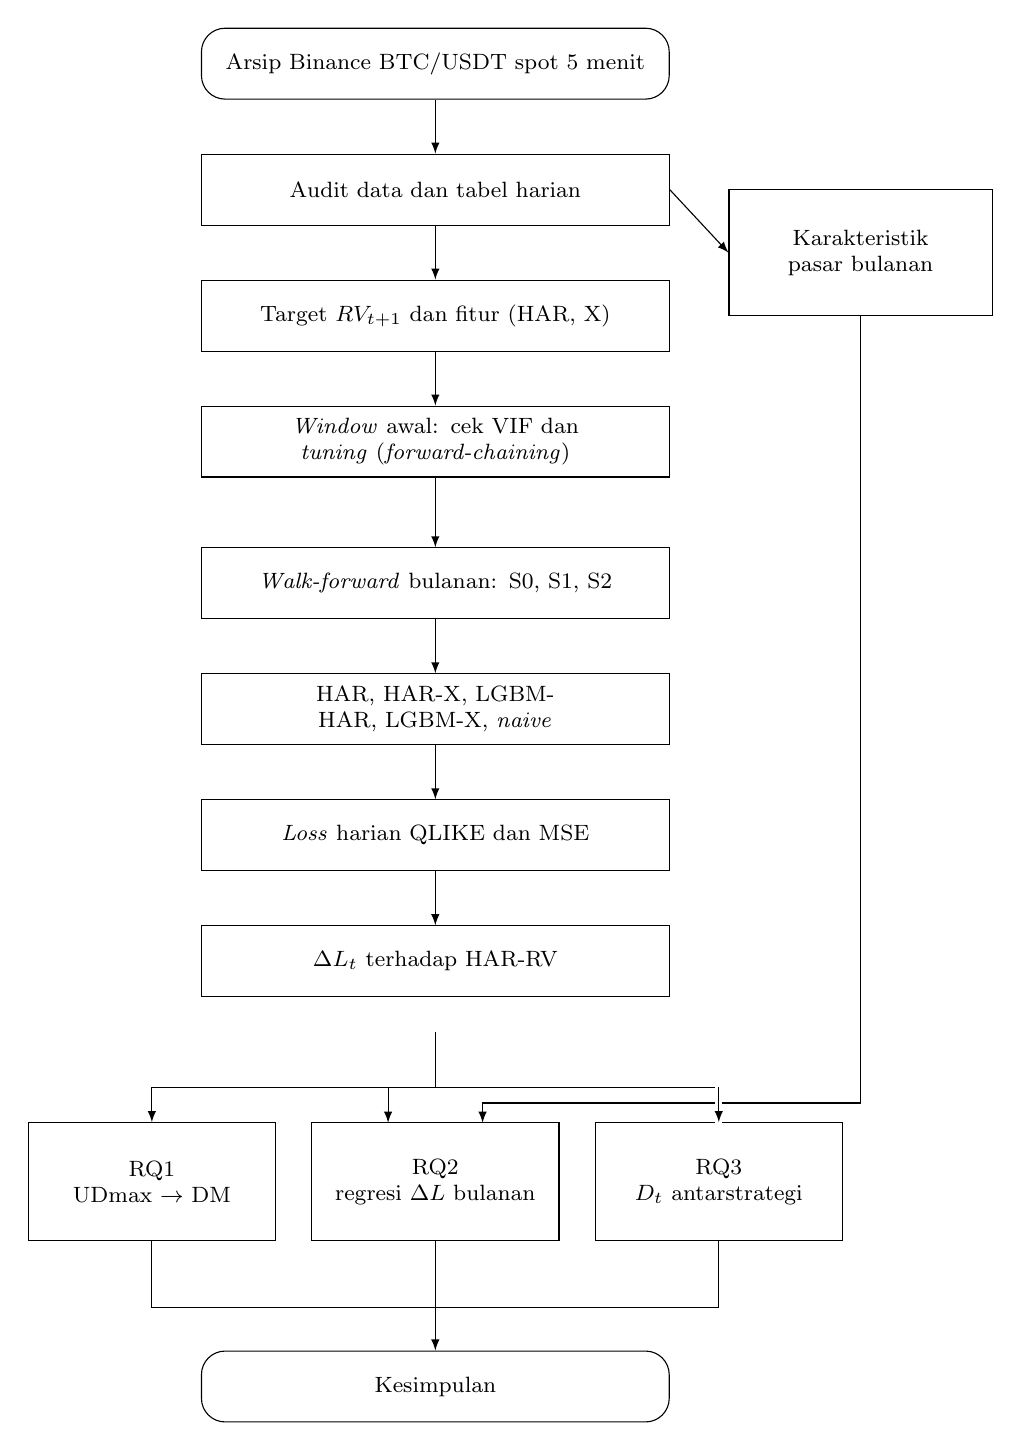
\begin{tikzpicture}[x=1mm,y=-1mm,
      kotak/.style={draw,align=center,inner sep=2pt,font=\footnotesize,
        text width=58mm,minimum height=9mm},
      ujung/.style={kotak,rounded corners=3mm},
      sisi/.style={draw,align=center,inner sep=2pt,font=\footnotesize,
        text width=32mm,minimum height=16mm},
      rq/.style={draw,align=center,inner sep=2pt,font=\footnotesize,
        text width=30mm,minimum height=15mm},
      pn/.style={->,>=latex}]

    % Kolom utama
    \node[ujung] (n1) at (0,0)
      {Arsip Binance BTC/USDT spot 5 menit};
    \node[kotak] (n2) at (0,16) {Audit data dan tabel harian};
    \node[kotak] (n3) at (0,32) {Target $RV_{t+1}$ dan fitur (HAR, X)};
    \node[kotak] (n4) at (0,48)
      {\textit{Window} awal: cek VIF dan \textit{tuning}
       (\textit{forward-chaining})};
    \node[kotak] (n5) at (0,66)
      {\textit{Walk-forward} bulanan: S0, S1, S2};
    \node[kotak] (n6) at (0,82)
      {HAR, HAR-X, LGBM-HAR, LGBM-X, \textit{naive}};
    \node[kotak] (n7) at (0,98) {\textit{Loss} harian QLIKE dan MSE};
    \node[kotak] (n8) at (0,114) {$\Delta L_t$ terhadap HAR-RV};

    % Masukan samping khusus RQ2
    \node[sisi] (pasar) at (54,24) {Karakteristik\\pasar bulanan};

    % Tiga rumusan masalah
    \node[rq] (rq1) at (-36,142) {RQ1\\UDmax $\rightarrow$ DM};
    \node[rq] (rq2) at (0,142) {RQ2\\regresi $\Delta L$ bulanan};
    \node[rq] (rq3) at (36,142) {RQ3\\$D_t$ antarstrategi};

    \node[ujung] (simp) at (0,168) {Kesimpulan};

    % Panah kolom utama
    \foreach \a/\b in {n1/n2, n2/n3, n3/n4, n4/n5, n5/n6, n6/n7, n7/n8}
      {\draw[pn] (\a) -- (\b);}

    % Audit data memasok karakteristik pasar bulanan
    \draw[pn] (n2.east) -- (pasar.west);

    % Satu panah dari delta L, lalu dibagikan ke ketiga RQ
    \draw (0,123) -- (0,130);
    \draw (-36,130) -- (36,130);
    \draw[pn] (-36,130) -- (rq1.north);
    \draw[pn] (-6,130) -- (-6,134.5);
    % Karakteristik pasar hanya memberi masukan ke RQ2; digambar lebih dulu
    % agar garis RQ3 di bawah tampak melompatinya.
    \draw[pn] (pasar.south) -- (54,132) -- (6,132) -- (6,134.5);
    \draw[white,line width=2.4pt] (36,130) -- (36,134.5);
    \draw[pn] (36,130) -- (rq3.north);

    % Ketiga RQ bermuara pada kesimpulan
    \draw (-36,149.5) -- (-36,158);
    \draw (0,149.5) -- (0,158);
    \draw (36,149.5) -- (36,158);
    \draw (-36,158) -- (36,158);
    \draw[pn] (0,158) -- (simp.north);
  \end{tikzpicture}
  \caption{Alur Penelitian}
  \label{fig:alur}
\end{figure}

\subsection{Tahap Uji Kelayakan}
Sebelum desain dikunci, dilakukan tahap uji kelayakan dengan pasangan
eksploratori LGBM-HAR dan HAR-RV. Tahap ini memeriksa kelengkapan data,
kebenaran \textit{pipeline}, kolinearitas fitur, prosedur \textit{tuning}, dan
daya uji. Pasangan konfirmatori LGBM-X terhadap HAR-RV tidak dievaluasi secara
\textit{out-of-sample} pada tahap tersebut, dan hasil uji kelayakan tidak
digunakan untuk mengubah rumusan masalah, hipotesis, maupun uji konfirmatori.

% CEK: tahap ini wajib diungkap terbuka (lihat hasil_eksperimen par. 5).
% Jangan menambahkan angka hasil pilot.

\subsection{Peralatan Penelitian}
Implementasi menggunakan bahasa Python 3.12 dengan pustaka \texttt{pandas},
\texttt{numpy}, \texttt{lightgbm} (versi 4 ke atas), \texttt{scikit-learn},
\texttt{statsmodels}, \texttt{scipy}, dan \texttt{matplotlib}. Estimator
kovarians HAC diimplementasikan sendiri mengikuti kernel Bartlett dengan
\textit{bandwidth} otomatis Andrews \cite{andrews1991} dan diverifikasi
menghasilkan nilai yang identik dengan fungsi \texttt{kernHAC} paket R
\texttt{sandwich}. Seluruh pelatihan memakai \textit{seed} tetap (42) dan mode
deterministik LightGBM.

% CEK: spesifikasi perangkat keras (laptop/OS) bila diminta pedoman; isi dari
% Ferdi.

\section{Desain Sistem}

\subsection{Data}
Data yang digunakan adalah \textit{klines} (OHLCV) BTC/USDT pasar spot dengan
resolusi 5 menit dari arsip publik Binance (\texttt{data.binance.vision}),
diunduh per bulan dan diverifikasi dengan \textit{checksum} SHA-256 resmi.
Periode data adalah 17 Agustus 2017, yaitu awal ketersediaan arsip, hingga
30 September 2026. Kolom yang digunakan adalah harga pembukaan, tertinggi,
terendah, penutupan, serta \textit{quote asset volume} (volume dalam USDT)
sebagai volume dolar. Ringkasan data ditunjukkan pada Tabel~\ref{tab:data} dan
pergerakannya pada Gambar~\ref{fig:data}.

\begin{table}[htbp]
  \caption{Ringkasan Data Penelitian}
  \label{tab:data}
  \centering
  \begingroup
  \setstretch{1}
  \begin{tabular}{|l|p{0.52\textwidth}|}
    \hline
    \textbf{Komponen} & \textbf{Keterangan} \\
    \hline
    Sumber & Binance Public Data, folder \textit{spot}, simbol berkas
      BTCUSDT \\
    \hline
    Resolusi & 5 menit (288 bar per hari UTC) \\
    \hline
    Periode & 17 Agustus 2017 -- 30 September 2026 \\
    \hline
    Jumlah bar & 957.865 \\
    \hline
    Jumlah hari & 3.332 \\
    \hline
    Hari dengan bar $<$ 95\% & 27 (dibuang, Subbab~\ref{subsec:audit}) \\
    \hline
    Hari dengan $RV = 0$ & 0 \\
    \hline
  \end{tabular}
  \endgroup
\end{table}

Pemilihan pasar spot didasarkan pada tiga alasan: histori spot tersedia sejak
2017 sementara kontrak \textit{perpetual} baru sejak sekitar September 2019,
padahal RQ3 membutuhkan data era awal; harga \textit{perpetual} mengandung
efek \textit{funding rate}, likuidasi, dan basis; serta keterbandingan dengan
literatur \cite{dudek2024}. Penggunaan satu bursa sepanjang periode juga
mencegah perubahan antarera tercampur dengan efek pergantian sumber data,
berbeda dengan Do yang berganti dari Bitstamp ke Binance pada November 2019
\cite{do2026}. Resolusi 5 menit dipilih sebagai kompromi yang aman lintas era
likuiditas (Subbab 2.2.3) \cite{liu2015}.

\begin{figure}[htbp]
  \centering
  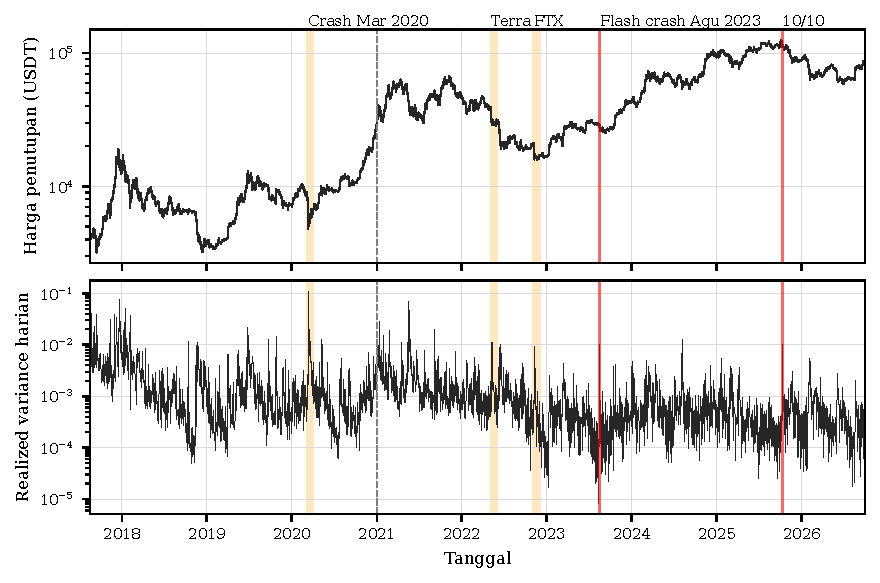
\includegraphics[width=\textwidth]{assets/gambar/gambar-3-2-harga-rv.pdf}
  \caption{Harga Penutupan dan \textit{Realized Variance} Harian BTC/USDT
    Spot, 17 Agustus 2017--30 September 2026}
  \label{fig:data}
\end{figure}

{\small Keterangan: garis putus-putus menandai batas era \textit{transition}
dan \textit{institutional} (1 Januari 2021) mengikuti Do \cite{do2026}; arsir
menandai \textit{crash} Maret 2020, Terra (Mei 2022), dan FTX (November 2022);
garis merah menandai \textit{flash crash} 17 Agustus 2023 dan 10 Oktober 2025
(``10/10''). Sumbu vertikal berskala logaritmik. Sumber: data Binance,
diolah.\par}

\subsection{Audit dan Pra-pemrosesan Data}
\label{subsec:audit}
Tahapan audit adalah sebagai berikut.
\begin{enumerate}
  \item \textbf{Standarisasi \textit{timestamp}.} Arsip Binance sejak
        1 Januari 2025 mencatat waktu dalam mikrodetik, sedangkan arsip
        sebelumnya dalam milidetik; seluruh \textit{timestamp} diseragamkan ke
        milidetik UTC, lalu duplikat dibuang dan data diurutkan.
  \item \textbf{Kelengkapan hari.} Hari dengan jumlah bar kurang dari 95\%
        (kurang dari 274 dari 288 bar) ditandai tidak lengkap. Pasangan
        observasi (fitur hari $t$, target hari $t+1$) dibuang bila hari $t$
        \textbf{atau} hari $t+1$ tidak lengkap atau memiliki RV nol. Sebanyak
        27 hari ditandai tidak lengkap. Sebagai uji sensitivitas, hari-hari
        tersebut dipertahankan.
  \item \textbf{Hari ekstrem dipertahankan} dan tidak dipangkas, karena
        lonjakan volatilitas justru bagian dari fenomena yang diteliti.
  \item \textbf{Volume nol.} Bar dengan volume dolar nol dikecualikan dari
        perhitungan Amihud (Persamaan~\eqref{eq:amihud}).
\end{enumerate}

\subsection{Target dan Fitur}
Target peramalan adalah $RV_{t+1}$ (Persamaan~\eqref{eq:rv}); model dilatih
pada $\ln RV_{t+1}$ lalu ramalannya dikembalikan ke skala level
(Subbab~\ref{subsec:teknis}). Seluruh fitur hari $t$ hanya memakai data hingga
akhir hari $t$. Tiga puluh hari pertama digunakan sebagai periode pemanasan
untuk rata-rata bulanan. Fitur dan model yang memakainya ditunjukkan pada
Tabel~\ref{tab:fitur}.

% CEK: $C_t$ pada baris return harian = harga penutupan bar terakhir hari $t$;
% sudah ditambahkan ke frontmatter/daftar-notasi.tex.
\begin{table}[htbp]
  \caption{Fitur dan Model Pemakainya}
  \label{tab:fitur}
  \centering
  \begingroup
  \setstretch{1}\small
  \begin{tabular}{|p{0.27\textwidth}|p{0.34\textwidth}|p{0.21\textwidth}|}
    \hline
    \textbf{Fitur} & \textbf{Definisi} & \textbf{Dipakai oleh} \\
    \hline
    $\ln RV_t$, $\ln RV^{(w)}_t$, $\ln RV^{(m)}_t$ &
    Persamaan~\eqref{eq:rata-rv}, rata-rata 1, 7, 30 hari & semua model \\
    \hline
    Proporsi semivarians negatif & $RS^-_t / RV_t$,
    Persamaan~\eqref{eq:semivarians} & HAR-X, LGBM-X \\
    \hline
    \textit{Return} harian & $\ln(C_t / C_{t-1})$ & HAR-X, LGBM-X \\
    \hline
    Log volume dolar & $\ln \sum_i QV_{t,i}$ & HAR-X, LGBM-X \\
    \hline
    Perubahan log volume dolar & selisih log volume dolar hari $t$ dan $t-1$ &
    HAR-X, LGBM-X \\
    \hline
    Log \textit{range} Parkinson & $\ln \sigma^2_{P,t}$,
    Persamaan~\eqref{eq:parkinson} & HAR-X, LGBM-X \\
    \hline
    Log Amihud & $\ln \text{Amihud}_t$, Persamaan~\eqref{eq:amihud} &
    LGBM-X \\
    \hline
  \end{tabular}
  \endgroup
\end{table}

Kolinearitas diperiksa dengan \textit{variance inflation factor} (VIF) pada
\textit{window} awal, sebelum fitur dikunci. Log Amihud (VIF 19,6) dan log
volume dolar (VIF 18,2) menunjukkan kolinearitas tinggi; secara konstruksi log
Amihud mendekati setengah $\ln RV$ dikurangi log volume dolar. Sesuai aturan
yang ditetapkan sebelumnya, log Amihud dibuang dari HAR-X saja, sehingga VIF
maksimum fitur X pada HAR-X menjadi 6,9. LGBM-X tetap memakai kesembilan fitur
karena model pohon tidak terpengaruh kolinearitas dalam estimasi.

\subsection{Model}
Model yang digunakan mengikuti desain $2 \times 2$ pada
Tabel~\ref{tab:desain}, ditambah model \textit{naive persistence}
$\widehat{RV}_{t+1} = RV_t$ sebagai pemeriksaan kewajaran.
\begin{itemize}
  \item \textbf{HAR-RV dan HAR-X} diestimasi dengan \textit{ordinary least
        squares} (OLS) pada $\ln RV_{t+1}$ (Persamaan~\eqref{eq:har}); HAR-X
        menambahkan fitur X sebagai regresor.
  \item \textbf{LGBM-HAR dan LGBM-X} menggunakan LightGBM \cite{ke2017} dengan
        \textit{objective} regresi kuadrat, \textit{bagging} 80\% data per
        pohon, dan \textit{hyperparameter} hasil \textit{tuning}
        (Subbab~\ref{subsec:tuning}).
  \item \textbf{Random Forest} dengan masukan yang sama dengan LGBM-X
        (300 pohon, minimum 20 observasi per daun, 33\% fitur per pemisahan)
        digunakan hanya sebagai uji sensitivitas jenis model pohon.
\end{itemize}

\subsection{Aturan Teknis Peramalan}
\label{subsec:teknis}
Aturan berikut berlaku sama untuk semua model.
\begin{enumerate}
  \item \textbf{Koreksi bias transformasi log.} Karena ramalan optimal di
        bawah QLIKE dan MSE adalah nilai harapan kondisional
        \cite{patton2011}, $\exp(\hat y)$ tanpa koreksi akan sistematis
        terlalu rendah. Ramalan dikoreksi menjadi
        $\exp(\hat y_{t+1} + \hat\sigma^2/2)$. Nilai $\hat\sigma^2$ adalah
        varians residual model yang dilatih pada 80\% awal \textit{window}
        latih, dihitung pada 20\% akhir \textit{window}; setelah itu model
        dilatih ulang pada seluruh \textit{window}. Residual
        \textit{in-sample} tidak dipakai karena LightGBM cenderung
        \textit{overfit}.
  \item \textbf{Batas bawah ramalan.} Ramalan dibatasi minimal sebesar
        persentil ke-1 target $RV$ pada \textit{window} latih,
        $\underline{F}$, karena QLIKE menghukum ramalan yang terlalu rendah
        jauh lebih berat \cite{patton2011}.
\end{enumerate}

Ramalan akhir adalah
\begin{equation}
  F_{t+1} = \max\!\left\{
    \exp\!\left(\hat y_{t+1} + \tfrac{1}{2}\hat\sigma^2\right),\;
    \underline{F} \right\}.
  \label{eq:ramalan}
\end{equation}
Sebagai uji sensitivitas, koreksi bias ditiadakan.

\subsection{\textit{Tuning Hyperparameter}}
\label{subsec:tuning}
\textit{Hyperparameter} LightGBM dituning \textbf{sekali} pada \textit{window}
awal (Agustus 2017 -- Agustus 2018) dengan validasi \textit{forward-chaining}
lima lipatan \cite{cerqueira2020}, lalu dikunci untuk seluruh periode
pengujian. Metrik pemilihan adalah rata-rata QLIKE ramalan $\exp(\hat y)$
antarlipatan. Bila kombinasi terbaik berada di tepi ruang pencarian untuk
\texttt{min\_child\_samples} atau \texttt{n\_estimators}, ruang pencarian
diperluas satu langkah ke arah tepi tersebut, maksimal dua kali, dengan batas
bawah \texttt{min\_child\_samples} sebesar 5 untuk menjaga regularisasi. Ruang
pencarian dan nilai terkunci ditunjukkan pada Tabel~\ref{tab:tuning}.

\begin{table}[htbp]
  \caption{Ruang Pencarian dan \textit{Hyperparameter} Terkunci}
  \label{tab:tuning}
  \centering
  \begingroup
  \setstretch{1}\small
  \begin{tabular}{|l|l|c|c|}
    \hline
    \textbf{Parameter} & \textbf{Ruang pencarian awal} & \textbf{LGBM-HAR} &
    \textbf{LGBM-X} \\
    \hline
    \texttt{num\_leaves} & 3, 7, 15 & 3 & 3 \\
    \hline
    \texttt{min\_child\_samples} & 10, 20, 40, 80 & 10 & 5 \\
    \hline
    \texttt{n\_estimators} & 50, 100, 300, 600 & 300 & 300 \\
    \hline
    \texttt{learning\_rate} & 0,03 & 0,03 & 0,03 \\
    \hline
    \texttt{reg\_lambda} & 1, 10 & 1 & 1 \\
    \hline
  \end{tabular}
  \endgroup
\end{table}

Nilai \texttt{min\_child\_samples} = 5 pada LGBM-X merupakan batas bawah ruang
pencarian yang ditetapkan sebelumnya, sehingga dicatat sebagai keputusan
desain untuk menjaga regularisasi.

\subsection{Skema Pembaruan Model (\textit{Walk-Forward})}
Peramalan dilakukan secara \textit{walk-forward} bulanan: pada awal setiap
bulan uji, model dilatih ulang (kecuali S0) menggunakan data dengan tanggal
target sebelum bulan tersebut, lalu meramalkan setiap hari dalam bulan itu.
Ketiga strategi utama mengikuti Tabel~\ref{tab:strategi} dan
Gambar~\ref{fig:strategi}. Model HAR-RV memakai strategi dan \textit{window}
yang sama dengan model ML pada setiap sel perbandingan \cite{chassot2026}.
Awal periode \textit{out-of-sample} setiap skema ditunjukkan pada
Tabel~\ref{tab:oos}; perbandingan antarskema selalu dilakukan pada periode
bersama.

\begin{table}[htbp]
  \caption{Skema Pembaruan dan Awal Periode \textit{Out-of-Sample}}
  \label{tab:oos}
  \centering
  \begingroup
  \setstretch{1}\small
  \begin{tabular}{|l|p{0.34\textwidth}|l|p{0.22\textwidth}|}
    \hline
    \textbf{Skema} & \textbf{Data latih} & \textbf{Awal OOS} &
    \textbf{Peran} \\
    \hline
    S0 & \textit{Window} awal, tidak dilatih ulang & 1 Sep 2018 &
    pembanding manfaat adaptasi \\
    \hline
    S1 & Seluruh data tersedia (\textit{expanding}) & 1 Sep 2018 &
    utama (RQ3) \\
    \hline
    S2-365 & 365 hari terakhir & 1 Sep 2018 & utama (RQ1, RQ2, RQ3) \\
    \hline
    S2-730 & 730 hari terakhir & 1 Sep 2019 & eksploratori \\
    \hline
    S2-180 & 180 hari terakhir & 1 Sep 2018 & eksploratori \\
    \hline
    S2-1095 & 1.095 hari terakhir & 1 Sep 2020 & eksploratori \\
    \hline
    Tertunda-365 & hari ke-730 s.d. ke-365 sebelum bulan uji & 1 Sep 2019 &
    eksploratori (umur data) \\
    \hline
  \end{tabular}
  \endgroup
\end{table}

Pembagian era mengikuti Do \cite{do2026}, dengan batas 1 Januari 2021 antara
era \textit{transition} dan \textit{institutional}; data tahun 2026
diperlakukan sebagai kelanjutan era \textit{institutional} dan diuji
sensitivitasnya. Batas era hanya digunakan dalam analisis, tidak sebagai fitur
model.

\subsection{Kontrol Kebocoran Data}
Langkah pencegahan kebocoran informasi masa depan:
\begin{enumerate}
  \item fitur hari $t$ hanya memakai data hingga akhir hari $t$, sedangkan
        target adalah hari $t+1$;
  \item \textit{tuning} hanya dilakukan pada \textit{window} awal dengan
        \textit{forward-chaining}, bukan validasi silang acak
        \cite{cerqueira2020};
  \item $\hat\sigma^2$ dan batas bawah $\underline{F}$ dihitung hanya dari
        \textit{window} latih;
  \item batas era tidak digunakan sebagai fitur;
  \item tidak ada ambang atau label yang dibentuk dengan melihat data
        \textit{out-of-sample}.
\end{enumerate}

\section{Perhitungan Manual}
Subbab ini memberikan contoh perhitungan satu kali peramalan untuk model
HAR-RV dan LGBM-HAR. Agar tidak memuat hasil pengujian, contoh diambil dari
\textit{window} awal: hari $t^* = $ 30 Agustus 2018 digunakan untuk meramalkan
$RV$ tanggal 31 Agustus 2018, dengan 339 observasi latih (tanggal target
16 September 2017 s.d. 30 Agustus 2018). Seluruh angka ditulis dengan enam
digit bermakna dan telah dicocokkan dengan keluaran implementasi.

\subsection{\textit{Realized Variance} dan Komponen HAR}
\textit{Return} bar pertama hari $t^*$ dihitung terhadap harga penutupan bar
terakhir 29 Agustus 2018, yaitu 7.031,22. Lima bar pertama ditunjukkan pada
Tabel~\ref{tab:manual-rv}.

\begin{table}[htbp]
  \caption{Lima Bar Pertama Hari $t^*$ dan Komponennya}
  \label{tab:manual-rv}
  \centering
  \begingroup
  \setstretch{1}\small
  \begin{tabular}{|l|r|r|r|c|}
    \hline
    \textbf{Waktu (UTC)} & \textbf{Penutupan} & \textbf{$r_{t,i}$} &
    \textbf{$r_{t,i}^2$} & \textbf{$r_{t,i} < 0$} \\
    \hline
    00:00 & 7.038,22 & $9{,}95065 \times 10^{-4}$ &
      $9{,}90153 \times 10^{-7}$ & tidak \\
    \hline
    00:05 & 7.036,24 & $-2{,}81361 \times 10^{-4}$ &
      $7{,}91638 \times 10^{-8}$ & ya \\
    \hline
    00:10 & 7.031,41 & $-6{,}86682 \times 10^{-4}$ &
      $4{,}71532 \times 10^{-7}$ & ya \\
    \hline
    00:15 & 7.039,17 & $1{,}10301 \times 10^{-3}$ &
      $1{,}21663 \times 10^{-6}$ & tidak \\
    \hline
    00:20 & 7.039,01 & $-2{,}27302 \times 10^{-5}$ &
      $5{,}16662 \times 10^{-10}$ & ya \\
    \hline
  \end{tabular}
  \endgroup
\end{table}

Penjumlahan kuadrat \textit{return} atas 288 bar (Persamaan~\eqref{eq:rv})
menghasilkan $RV_{t^*} = 5{,}37199 \times 10^{-4}$. Sebanyak 154 bar memiliki
\textit{return} negatif, sehingga $RS^-_{t^*} = 2{,}67476 \times 10^{-4}$
(Persamaan~\eqref{eq:semivarians}) dan proporsinya
$RS^-_{t^*}/RV_{t^*} = 0{,}497908$.

Komponen HAR dihitung dari rata-rata RV harian, mingguan, dan bulanan
(Persamaan~\eqref{eq:rata-rv}) seperti pada Tabel~\ref{tab:manual-har}.

\begin{table}[htbp]
  \caption{Komponen HAR pada Hari $t^*$}
  \label{tab:manual-har}
  \centering
  \begingroup
  \setstretch{1}\small
  \begin{tabular}{|l|l|}
    \hline
    \textbf{Komponen} & \textbf{Nilai} \\
    \hline
    RV 24 Agustus 2018 & $6{,}28396 \times 10^{-4}$ \\
    \hline
    RV 25 Agustus 2018 & $3{,}50138 \times 10^{-4}$ \\
    \hline
    RV 26 Agustus 2018 & $4{,}82313 \times 10^{-4}$ \\
    \hline
    RV 27 Agustus 2018 & $4{,}99351 \times 10^{-4}$ \\
    \hline
    RV 28 Agustus 2018 & $4{,}54143 \times 10^{-4}$ \\
    \hline
    RV 29 Agustus 2018 & $4{,}40669 \times 10^{-4}$ \\
    \hline
    RV 30 Agustus 2018 ($=RV_{t^*}$) & $5{,}37199 \times 10^{-4}$ \\
    \hline
    Rata-rata mingguan $RV^{(w)}_{t^*}$ & $4{,}84601 \times 10^{-4}$ \\
    \hline
    Bulanan (30 nilai, 1--30 Agustus 2018): minimum &
      $3{,}50138 \times 10^{-4}$ \\
    \hline
    \phantom{Bulanan (30 nilai, 1--30 Agustus 2018): }maksimum &
      $3{,}80630 \times 10^{-3}$ \\
    \hline
    Rata-rata bulanan $RV^{(m)}_{t^*}$ & $1{,}27306 \times 10^{-3}$ \\
    \hline
    $\ln RV_{t^*}$ & $-7{,}52914$ \\
    \hline
    $\ln RV^{(w)}_{t^*}$ & $-7{,}63218$ \\
    \hline
    $\ln RV^{(m)}_{t^*}$ & $-6{,}66633$ \\
    \hline
  \end{tabular}
  \endgroup
\end{table}

\subsection{Fitur X}
Keenam fitur X pada hari $t^*$ ditunjukkan pada Tabel~\ref{tab:manual-x}.
Model HAR-X tidak memakai log Amihud, sesuai hasil pemeriksaan VIF pada
Subbab~\ref{subsec:audit}; fitur tersebut hanya dipakai LGBM-X.

\begin{table}[htbp]
  \caption{Fitur X pada Hari $t^*$}
  \label{tab:manual-x}
  \centering
  \begingroup
  \setstretch{1}\small
  \begin{tabular}{|p{0.26\textwidth}|p{0.34\textwidth}|p{0.26\textwidth}|}
    \hline
    \textbf{Fitur} & \textbf{Masukan mentah} & \textbf{Hasil} \\
    \hline
    \textit{Return} harian & penutupan $t^*$ = 6.984,84; penutupan $t^*-1$ =
      7.031,22 & $-0{,}00661815$ \\
    \hline
    Log volume dolar & volume dolar $t^*$ = $3{,}09357 \times 10^{8}$ &
      19,5500 \\
    \hline
    Perubahan log volume dolar & volume dolar $t^*-1$ =
      $3{,}04565 \times 10^{8}$ & $19{,}5500 - 19{,}5344 = 0{,}0156107$ \\
    \hline
    Log \textit{range} Parkinson & $P^H_{t^*}$ = 7.063,63;
      $P^L_{t^*}$ = 6.784,81 & $-7{,}44394$ \\
    \hline
    Log Amihud & $10^6 \times$ rata-rata $|r_{t,i}|/QV_{t,i}$ =
      $0{,}00116494$ & $-6{,}75508$ \\
    \hline
    Proporsi semivarians negatif & lihat Subbab 3.3.1 & 0,497908 \\
    \hline
  \end{tabular}
  \endgroup
\end{table}

\subsection{Peramalan HAR-RV dan LGBM-HAR}
Koefisien HAR-RV hasil OLS pada \textit{window} latih adalah
$\beta_0 = -0{,}569890$, $\beta_d = 0{,}478542$, $\beta_w = 0{,}0689003$, dan
$\beta_m = 0{,}384379$. Dengan Persamaan~\eqref{eq:har},
\begin{align}
  \hat y_{t^*+1} &= (-0{,}569890)
    + (0{,}478542)(-7{,}52914)
    + (0{,}0689003)(-7{,}63218) \nonumber \\
  &\quad + (0{,}384379)(-6{,}66633) \nonumber \\
  &= (-0{,}569890) + (-3{,}60301) + (-0{,}525859) + (-2{,}56240) \nonumber \\
  &= -7{,}26116 .
  \label{eq:manual-har}
\end{align}
Varians residual $\hat\sigma^2 = 0{,}497938$ diperoleh dari model yang dilatih
pada 271 observasi awal dan dievaluasi pada 68 observasi akhir. Dengan
Persamaan~\eqref{eq:ramalan},
$\exp(-7{,}26116 + 0{,}248969) = 9{,}00836 \times 10^{-4}$, yang berada di
atas batas bawah $\underline{F} = 2{,}90955 \times 10^{-4}$, sehingga
$F_{\text{HAR}} = 9{,}00836 \times 10^{-4}$.

Pada LGBM-HAR, nilai awal berupa rata-rata $\ln RV_{t+1}$ data latih,
$-6{,}03756$, dilebur ke nilai daun pohon pertama, sehingga $\hat y$ merupakan
jumlah nilai daun dari 300 pohon (Persamaan~\eqref{eq:gbdt}). Struktur dua
pohon pertama beserta lintasan hari $t^*$ ditunjukkan pada
Gambar~\ref{fig:manual-pohon}.

% CEK: jumlah n per daun pohon ke-1 (256) tidak konsisten dengan bagging 80%
% dari 339 obs (~271); sedang dicek di chat script. Karena itu n tidak
% ditampilkan.
\begin{figure}[htbp]
  \centering
  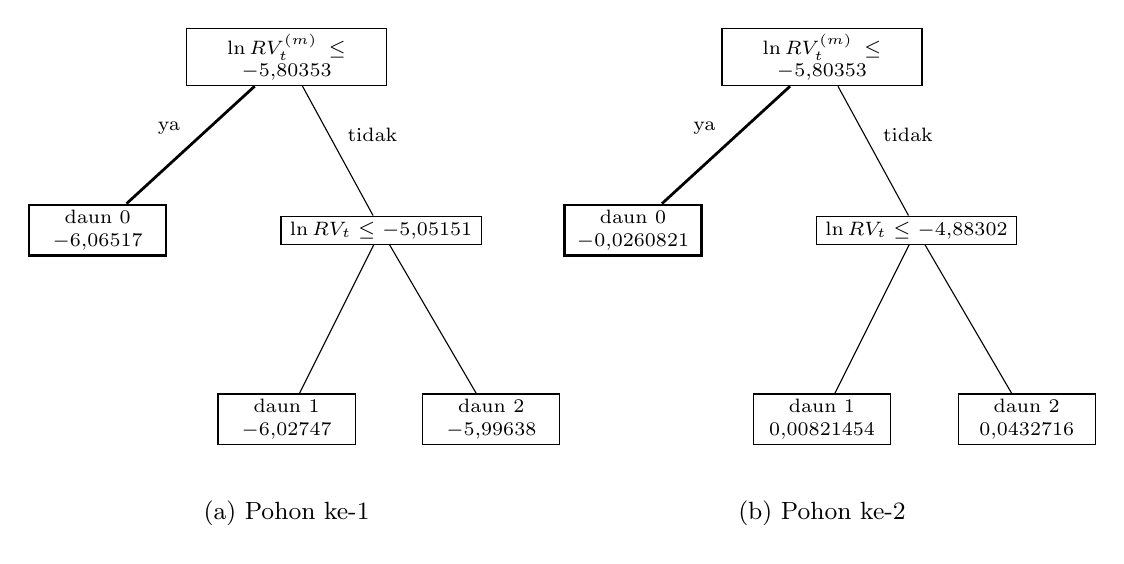
\begin{tikzpicture}[x=1mm,y=-1mm,
      simpul/.style={draw,align=center,inner sep=2pt,font=\scriptsize,
        text width=24mm},
      daun/.style={draw,align=center,inner sep=2pt,font=\scriptsize,
        text width=16mm},
      tebal/.style={line width=1pt}]

    % Panel kiri: pohon ke-1
    \begin{scope}
      \node[simpul] (a) at (30,0) {$\ln RV^{(m)}_t \le -5{,}80353$};
      \node[daun,tebal] (a0) at (6,22) {daun 0\\$-6{,}06517$};
      \node[simpul] (a1) at (42,22) {$\ln RV_t \le -5{,}05151$};
      \node[daun] (a11) at (30,46) {daun 1\\$-6{,}02747$};
      \node[daun] (a12) at (56,46) {daun 2\\$-5{,}99638$};
      \draw[tebal] (a) -- node[above left,font=\scriptsize] {ya} (a0);
      \draw (a) -- node[above right,font=\scriptsize] {tidak} (a1);
      \draw (a1) -- (a11);
      \draw (a1) -- (a12);
      \node[font=\small] at (30,58) {(a) Pohon ke-1};
    \end{scope}

    % Panel kanan: pohon ke-2
    \begin{scope}[xshift=68mm]
      \node[simpul] (b) at (30,0) {$\ln RV^{(m)}_t \le -5{,}80353$};
      \node[daun,tebal] (b0) at (6,22) {daun 0\\$-0{,}0260821$};
      \node[simpul] (b1) at (42,22) {$\ln RV_t \le -4{,}88302$};
      \node[daun] (b11) at (30,46) {daun 1\\$0{,}00821454$};
      \node[daun] (b12) at (56,46) {daun 2\\$0{,}0432716$};
      \draw[tebal] (b) -- node[above left,font=\scriptsize] {ya} (b0);
      \draw (b) -- node[above right,font=\scriptsize] {tidak} (b1);
      \draw (b1) -- (b11);
      \draw (b1) -- (b12);
      \node[font=\small] at (30,58) {(b) Pohon ke-2};
    \end{scope}
  \end{tikzpicture}
  \caption{Struktur Pohon ke-1 dan ke-2 LGBM-HAR pada Contoh Perhitungan}
  \label{fig:manual-pohon}
  \sumber{Garis tebal menandai lintasan hari $t^*$, dengan
    $\ln RV^{(m)}_{t^*} = -6{,}66633$}
\end{figure}

Hari $t^*$ memiliki $\ln RV^{(m)}_{t^*} = -6{,}66633$, yang memenuhi syarat
pemisahan pertama pada kedua pohon, sehingga keduanya berakhir di daun 0.
Kontribusi pohon ke-1 adalah $-6{,}06517$, yaitu gabungan nilai awal
$-6{,}03756$ dan nilai daun $-0{,}0276166$; kontribusi pohon ke-2 adalah
$-0{,}0260821$; dan jumlah kontribusi pohon ke-3 hingga ke-300 adalah
$-1{,}22919$. Total ketiganya menghasilkan $\hat y_{t^*+1} = -7{,}32044$.
Dengan $\hat\sigma^2 = 0{,}511547$, diperoleh
$\exp(-7{,}32044 + 0{,}255773) = 8{,}54778 \times 10^{-4}$, yang juga di atas
batas bawah, sehingga $F_{\text{LGBM}} = 8{,}54778 \times 10^{-4}$.

\subsection{Evaluasi Satu Hari}
\textit{Realized variance} aktual tanggal 31 Agustus 2018 adalah
$4{,}14190 \times 10^{-4}$. Nilai \textit{loss} kedua model dihitung dengan
Persamaan~\eqref{eq:loss} dan ditunjukkan pada Tabel~\ref{tab:manual-loss}.

\begin{table}[htbp]
  \caption{Evaluasi Ramalan 31 Agustus 2018}
  \label{tab:manual-loss}
  \centering
  \begingroup
  \setstretch{1}\small
  \begin{tabular}{|l|l|l|l|l|}
    \hline
    \textbf{Model} & \textbf{$F_{t+1}$} & \textbf{$RV_{t+1}/F_{t+1}$} &
    \textbf{QLIKE} & \textbf{MSE} \\
    \hline
    HAR-RV & $9{,}00836 \times 10^{-4}$ & 0,459784 & 0,236783 &
      $2{,}36825 \times 10^{-7}$ \\
    \hline
    LGBM-HAR & $8{,}54778 \times 10^{-4}$ & 0,484558 & 0,209076 &
      $1{,}94118 \times 10^{-7}$ \\
    \hline
  \end{tabular}
  \endgroup
\end{table}

Selisih \textit{loss} pada hari tersebut (Persamaan~\eqref{eq:delta-loss})
adalah $\Delta L = 0{,}209076 - 0{,}236783 = -0{,}0277067$. Nilai negatif
menunjukkan LGBM-HAR lebih akurat \textbf{pada hari contoh ini saja}; satu
hari tidak dapat dijadikan dasar kesimpulan, sehingga pengujian dilakukan atas
seluruh periode \textit{out-of-sample} sebagaimana diuraikan pada Subbab 3.4.

\section{Evaluasi dan Pengujian Hipotesis}

\subsection{Fungsi \textit{Loss} dan Selisih \textit{Loss}}
Setiap ramalan dievaluasi dengan QLIKE sebagai \textit{loss} utama dan MSE
pada skala level sebagai pelengkap (Persamaan~\eqref{eq:loss}). Objek analisis
adalah selisih \textit{loss} harian $\Delta L_t$
(Persamaan~\eqref{eq:delta-loss}). Pasangan konfirmatori adalah LGBM-X
terhadap HAR-RV pada skema S2-365; pasangan lain, yaitu LGBM-HAR--HAR,
HAR-X--HAR, LGBM-X--LGBM-HAR, dan LGBM-X--HAR-X, digunakan untuk dekomposisi
secara eksploratori.

\subsection{Uji Konfirmatori}
Uji konfirmatori setiap hipotesis mengikuti Tabel~\ref{tab:ringkasan}.
Rincian pelaksanaannya adalah sebagai berikut.
\begin{enumerate}
  \item \textbf{RQ1.} UDmax (Persamaan~\eqref{eq:udmax}) pada rata-rata
        $\Delta L_t$ dengan \textit{trimming} $\varepsilon = 0{,}15$ dan
        maksimum lima perubahan, statistik Wald memakai kovarians HAC
        \cite{bai1998,bai2003,martins2016}. Bila UDmax tidak menolak $H_0$,
        dilanjutkan dengan uji tipe Diebold--Mariano
        (Persamaan~\eqref{eq:dm}) pada seluruh sampel.
  \item \textbf{RQ2.} H2a diuji dengan regresi rata-rata $\Delta L$ bulanan
        pada empat karakteristik pasar (Subbab~\ref{subsec:rq2var}), dengan
        uji-F bersama berbasis kovarians HAC. H2b diuji dengan regresi
        $\Delta L_t = \alpha + \delta\,\text{Era}_t + e_t$ untuk dua
        pasangan kontribusi fitur X (HAR-X--HAR dan LGBM-X--LGBM-HAR), uji-t
        HAC pada $\delta$, dengan koreksi Holm atas dua uji tersebut
        \cite{holm1979}.
  \item \textbf{RQ3.} Uji-t HAC dua sisi pada rata-rata $D_t$ (Subbab 2.4) di
        era \textit{institutional}, pada periode bersama S2-365 dan S1. H3
        didukung bila rata-rata $D_t$ negatif dan signifikan; rata-rata
        positif yang signifikan dibaca sebagai dukungan bagi hipotesis
        tandingan.
\end{enumerate}

Semua uji menggunakan taraf signifikansi 5\% dan kovarians HAC Newey--West
dengan kernel Bartlett dan \textit{bandwidth} otomatis Andrews
\cite{newey1987,andrews1991}.

Nilai kritis UDmax, uji perubahan berurutan, dan \textit{Fluctuation test}
diperoleh dengan simulasi Monte Carlo, bukan dikutip dari tabel: 3.000
replikasi deret normal baku sepanjang 1.000 observasi untuk UDmax, dan 5.000
replikasi gerak Brown diskret untuk \textit{Fluctuation test}.
\textit{p-value} dihitung sebagai $(R^{+}+1)/(R+1)$, dengan $R^{+}$ jumlah
statistik simulasi yang tidak lebih kecil dari statistik amatan dan $R$ jumlah
replikasi. Nilai kritis simulasi dibandingkan
dengan tabel Bai--Perron sebagai pemeriksaan \cite{bai1998}.

% CEK: tabel asli Bai--Perron (1998) untuk q = 1, epsilon = 0,15 belum
% dicocokkan langsung.

\subsection{Variabel Karakteristik Pasar (RQ2)}
\label{subsec:rq2var}
Untuk setiap bulan uji dihitung empat variabel seperti pada
Tabel~\ref{tab:rq2var}.

\begin{table}[htbp]
  \caption{Variabel Karakteristik Pasar Bulanan}
  \label{tab:rq2var}
  \centering
  \begingroup
  \setstretch{1}\small
  \begin{tabular}{|p{0.3\textwidth}|p{0.55\textwidth}|}
    \hline
    \textbf{Variabel} & \textbf{Definisi} \\
    \hline
    Level volatilitas & rata-rata $\ln RV_t$ dalam bulan \\
    \hline
    Volatilitas dari volatilitas & deviasi standar $\ln RV_t$ dalam bulan \\
    \hline
    Likuiditas & rata-rata \textit{spread} Abdi--Ranaldo harian
      \cite{abdi2017} \\
    \hline
    Pergeseran distribusi fitur & rata-rata $D^{\text{KS}}$
      (Persamaan~\eqref{eq:ks}) antara \textit{window} latih S2-365 dan bulan
      uji atas sembilan fitur LGBM-X \\
    \hline
  \end{tabular}
  \endgroup
\end{table}

\textit{Spread} Abdi--Ranaldo harian dihitung sebagai
\begin{equation}
  s_t = \sqrt{\max\{4\,(c_t - \bar{p}_t)(c_t - \bar{p}_{t+1}),\, 0\}},
  \label{eq:abdi}
\end{equation}
dengan $\bar{p}_t = (\ln P^H_t + \ln P^L_t)/2$ dan $c_t$ logaritma harga
penutupan hari $t$. Nilai negatif di bawah akar dijadikan nol sebelum
dirata-rata. Sebagai uji sensitivitas, estimator Corwin--Schultz
\cite{corwin2012} digunakan sebagai pengganti. Sebagai pelengkap deskriptif,
dihitung pula \textit{population stability index} (PSI) antara \textit{window}
latih dan bulan uji.

Regresi H2a dirumuskan sebagai
\begin{equation}
  \overline{\Delta L}_\tau = \alpha + \sum_{k=1}^{4} \gamma_k\, z_{k,\tau}
    + \delta\, \text{Era}_\tau + u_\tau,
  \label{eq:rq2}
\end{equation}
dengan $\overline{\Delta L}_\tau$ rata-rata $\Delta L_t$ bulan $\tau$,
$z_{k,\tau}$ keempat variabel pada Tabel~\ref{tab:rq2var}, dan
$\text{Era}_\tau$ variabel \textit{dummy} era \textit{institutional} yang
selalu disertakan. Untuk menghindari regresi palsu, setiap regresor diuji
dengan ADF \cite{dickey1979} dan KPSS \cite{kwiatkowski1992}; regresor
di-\textit{differencing} bila ADF gagal menolak akar unit ($p > 0{,}05$)
\textbf{dan} KPSS menolak stasioneritas ($p < 0{,}05$). Hipotesis yang diuji
adalah $\gamma_1 = \gamma_2 = \gamma_3 = \gamma_4 = 0$. Interpretasi bersifat
asosiatif, bukan kausal.

\subsection{Analisis Eksploratori}
Analisis berikut bersifat eksploratori dan \textit{p-value}-nya dikoreksi
dengan prosedur Holm per keluarga rumusan masalah \cite{holm1979}:
\begin{enumerate}
  \item uji perubahan berurutan $\sup F(\ell+1 \mid \ell)$ untuk menentukan
        jumlah dan tanggal perubahan \cite{bai2003};
  \item \textit{Fluctuation test} dengan $\mu = 0{,}3$ dan $0{,}2$ sebagai
        grafik deskriptif \cite{giacomini2010};
  \item pasangan dekomposisi, skema S0 dan S2 lain, serta \textit{loss} MSE;
  \item kurva panjang \textit{window} (S2-180 s.d. S1) dan perbandingan efek
        jumlah data (S2-730 terhadap S2-365) dengan efek umur data
        (Tertunda-365 terhadap S2-365);
  \item analisis daya UDmax dengan \textit{bootstrap} blok 30 hari.
\end{enumerate}

\subsection{Uji Sensitivitas}
Kesimpulan konfirmatori diperiksa terhadap variasi pada
Tabel~\ref{tab:sensitivitas}.

% CEK: sensitivitas RV 5 menit subsampled (butuh data 1 menit) dan retuning
% tahunan ada di rencana v2.5 tetapi belum dijalankan. Tambahkan ke tabel
% hanya jika Ferdi memutuskan akan menjalankannya.
\begin{table}[htbp]
  \caption{Variasi Uji Sensitivitas}
  \label{tab:sensitivitas}
  \centering
  \begingroup
  \setstretch{1}\small
  \begin{tabular}{|p{0.3\textwidth}|p{0.55\textwidth}|}
    \hline
    \textbf{Variasi} & \textbf{Perubahan terhadap desain utama} \\
    \hline
    Tanpa 2026 & data uji dibatasi hingga 31 Desember 2025 \\
    \hline
    Hari tidak lengkap dipertahankan & aturan audit
      Subbab~\ref{subsec:audit} butir 2 tidak diterapkan \\
    \hline
    \textit{Window} awal 24 bulan & \textit{tuning} dan awal OOS memakai
      \textit{window} awal 730 hari \\
    \hline
    Lag 1, 5, 22 & horizon HAR mengikuti hari perdagangan saham \\
    \hline
    Random Forest & LGBM-X diganti Random Forest \\
    \hline
    RV 15 menit & target dan fitur HAR dari \textit{return} 15 menit \\
    \hline
    Tanpa koreksi bias & $\hat\sigma^2 = 0$ pada
      Persamaan~\eqref{eq:ramalan} \\
    \hline
    HAR re-estimasi harian & HAR dilatih ulang setiap hari, bukan bulanan \\
    \hline
    Likuiditas Corwin--Schultz & khusus H2a \\
    \hline
  \end{tabular}
  \endgroup
\end{table}

\section{Jadwal Penelitian}
Jadwal pelaksanaan penelitian ditunjukkan pada Tabel~\ref{tab:jadwal}.

% CEK: kolom bulan dan tanda centang diisi Ferdi sesuai rencana dan kalender
% prodi. Jangan menebak durasi.
\begin{table}[htbp]
  \caption{Jadwal penelitian}
  \label{tab:jadwal}
  \centering
  \begingroup
  \setstretch{1}
  \begin{tabular}{|c|p{0.45\textwidth}|c|c|c|c|}
    \hline
    \textbf{No} & \textbf{Kegiatan} & \textbf{Bln 1} & \textbf{Bln 2} &
    \textbf{Bln 3} & \textbf{Bln 4} \\
    \hline
    1 & Studi literatur dan verifikasi kebaruan & & & & \\
    \hline
    2 & Pengumpulan dan audit data & & & & \\
    \hline
    3 & Uji kelayakan (\textit{pilot}) & & & & \\
    \hline
    4 & Implementasi \textit{pipeline} dan eksperimen & & & & \\
    \hline
    5 & Analisis dan pengujian hipotesis & & & & \\
    \hline
    6 & Penulisan Bab IV dan V & & & & \\
    \hline
    7 & Seminar hasil dan sidang & & & & \\
    \hline
  \end{tabular}
  \endgroup
\end{table}
